\documentclass[10pt]{beamer}
\usetheme[
%%% option passed to the outer theme
%    progressstyle=fixedCircCnt,   % fixedCircCnt, movingCircCnt (moving is deault)
  ]{Feather}
  
% If you want to change the colors of the various elements in the theme, edit and uncomment the following lines

% Change the bar colors:
%\setbeamercolor{Feather}{fg=red!20,bg=red}

% Change the color of the structural elements:
%\setbeamercolor{structure}{fg=red}

% Change the frame title text color:
%\setbeamercolor{frametitle}{fg=blue}

% Change the normal text color background:
%\setbeamercolor{normal text}{fg=black,bg=gray!10}

\setbeamertemplate{caption}[numbered]
\setbeamertemplate{section in toc}[sections numbered]
\setbeamertemplate{subsection in toc}[square]
%\setbeamertemplate{bibliography item}{\insertbiblabel}
\setbeamertemplate{bibliography item}[article]
\setbeamertemplate{navigation symbols}{}


%\useoutertheme{miniframes}

%-------------------------------------------------------
% INCLUDE PACKAGES
%-------------------------------------------------------

\usepackage[utf8]{inputenc}
\usepackage[english]{babel}
\usepackage[T1]{fontenc}
\usepackage{helvet}

\usepackage{tabu}
\usepackage{booktabs}
\usepackage[shortlabels]{enumitem}

%-------------------------------------------------------
% DEFINING AND REDEFINING COMMANDS
%-------------------------------------------------------

% colored hyperlinks
\newcommand{\chref}[2]{
  \href{#1}{{\usebeamercolor[bg]{Feather}#2}}
}

\renewcommand{\logofile}{images/TUD}

\setitemize{label=\usebeamerfont*{itemize item}%
  \usebeamercolor[fg]{itemize item}
  \usebeamertemplate{itemize item}}

%-------------------------------------------------------
% INFORMATION IN THE TITLE PAGE
%-------------------------------------------------------

\title[] % [] is optional - is placed on the bottom of the sidebar on every slide
{ % is placed on the title page
      \textbf{Animal Biometrics}
}

\subtitle[Visual Computing Praktikum -- SS 2018]
{
      \textbf{Visual Computing Praktikum -- SS 2018}
}

\author[Fabian Otto]
{      Fabian Otto \\
      {\ttfamily fabian.otto@stud.tu-darmstadt.de}\\
}

\institute[Technische Universit\"at Darmstadt]
{
      
      Graphical Interactive Systems\\
      Technische Universit\"at Darmstadt\\
      [\medskipamount]
      
\includegraphics[scale=.12]{images/TUD}%
  %there must be an empty line above this line - otherwise some unwanted space is added between the university and the country (I do not know why;( )
}

\logo{
       
\includegraphics[scale=.03]{images/TUD}%
}

\date{\today}

%\AtBeginSection[]
%{
% \begin{frame}<beamer>
% \frametitle{Inhaltsverzeichnis}
% \tableofcontents[currentsection]
% \end{frame}
%}

%-------------------------------------------------------
% THE BODY OF THE PRESENTATION
%-------------------------------------------------------

\begin{document}

%-------------------------------------------------------
% THE TITLEPAGE
%-------------------------------------------------------

{\1
\begin{frame}[plain, noframenumbering] 
  \titlepage 
\end{frame}}

\begin{frame}{Outline}{}
\tableofcontents
\end{frame}

\AtBeginSection[]
{
	\begin{frame}{Outline}
		\tableofcontents[currentsection]
	\end{frame}
}

%-------------------------------------------------------
\section{Introduction and Motivation}
%-------------------------------------------------------

\begin{frame}{Introduction and Motivation}
	\centering
	Insert image of Animal Biometrics here 
\end{frame}

%-------------------------------------------------------
\section{Problem 1: Classification of Individuals}
%-------------------------------------------------------
\subsection{Data Set}
%-------------------------------------------------------
\begin{frame}{Data Set}
	\begin{minipage}[c]{0.48\linewidth}
		\centering
		\begin{figure}
			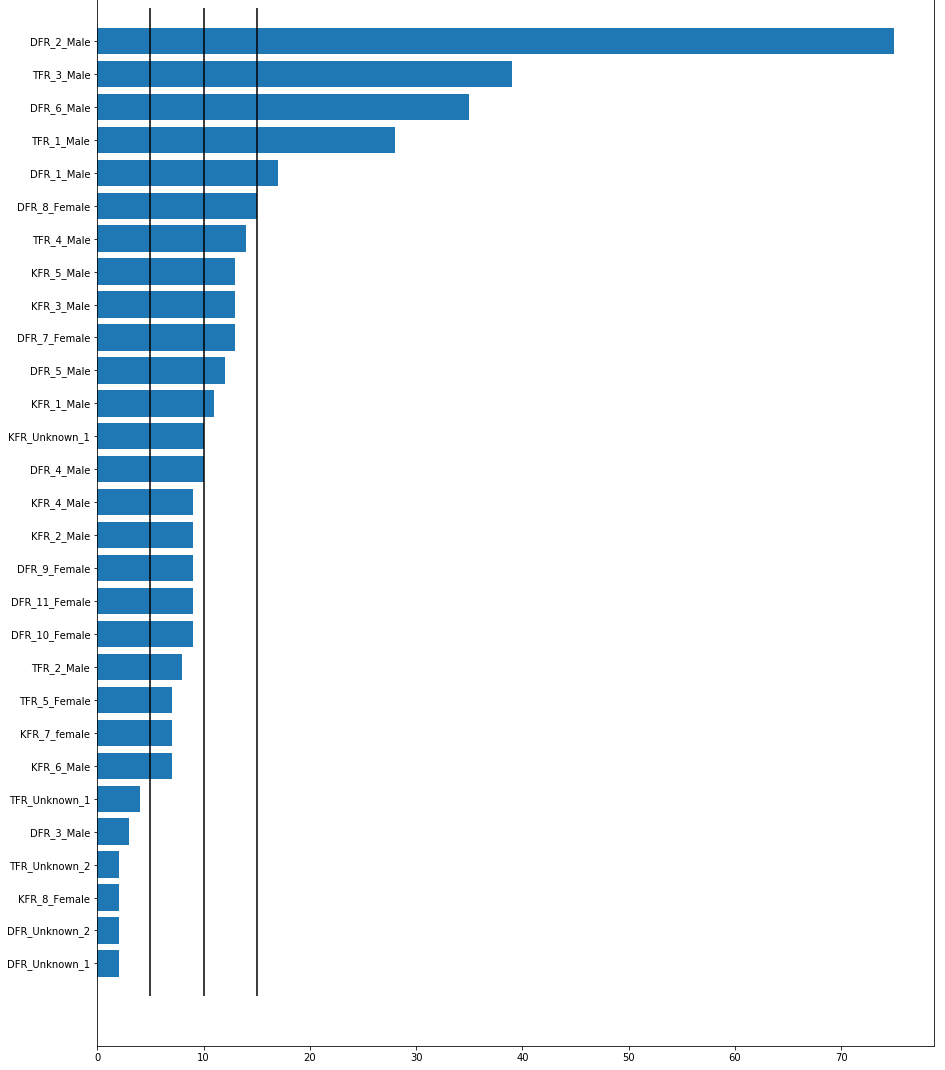
\includegraphics[width=\linewidth,height=.8\textheight,keepaspectratio]{images/Data_dist_leo_lines_sorted_hori.png}
			\caption{ResNet Architecure}
		\end{figure}
	\end{minipage}
	\hfill
	\begin{minipage}[c]{0.48\linewidth}
		\begin{itemize}
			\item Uneven data distribution (3 to 99 images per class)
			\item 29 classes/Individuals
			\item Low quality image from camera traps
		\end{itemize}
	\end{minipage}
\end{frame}

%-------------------------------------------------------

\begin{frame}{Good Example Images}		
	\centering
	\begin{minipage}[c]{0.48\linewidth}
		\begin{figure}
			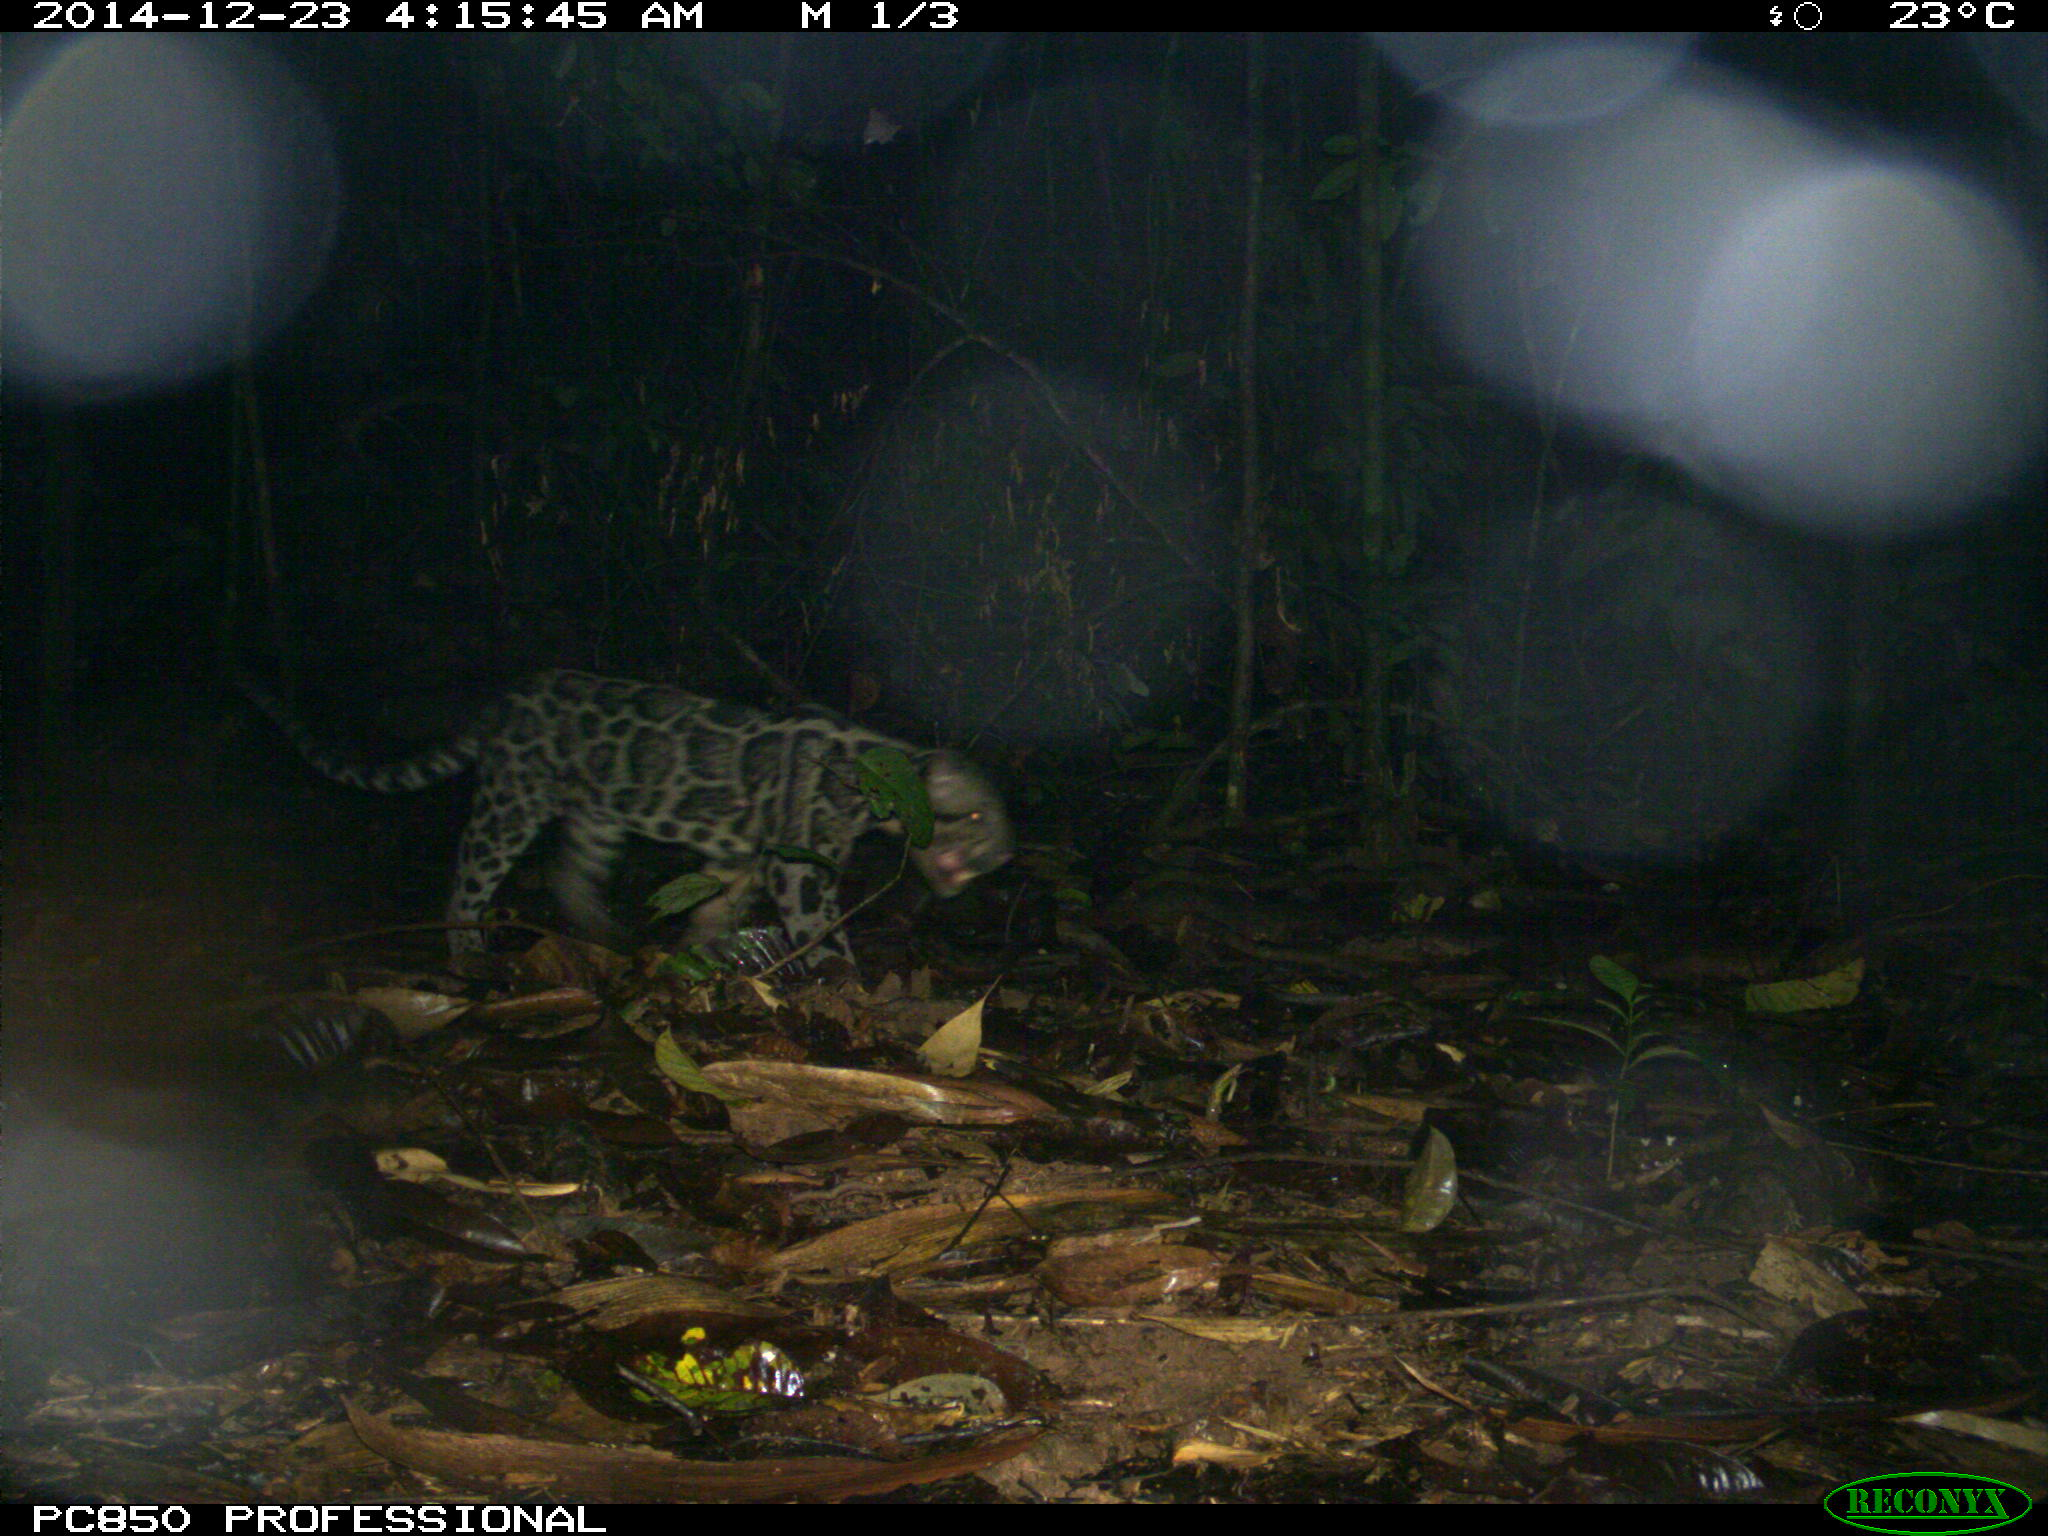
\includegraphics[width=\linewidth,height=\textheight,keepaspectratio]{images/example_DFR_2_male.JPG}
			\caption{DFR 2 Male}
		\end{figure}
	\end{minipage}
	\hfill
	\begin{minipage}[c]{0.48\linewidth}
		\begin{figure}
			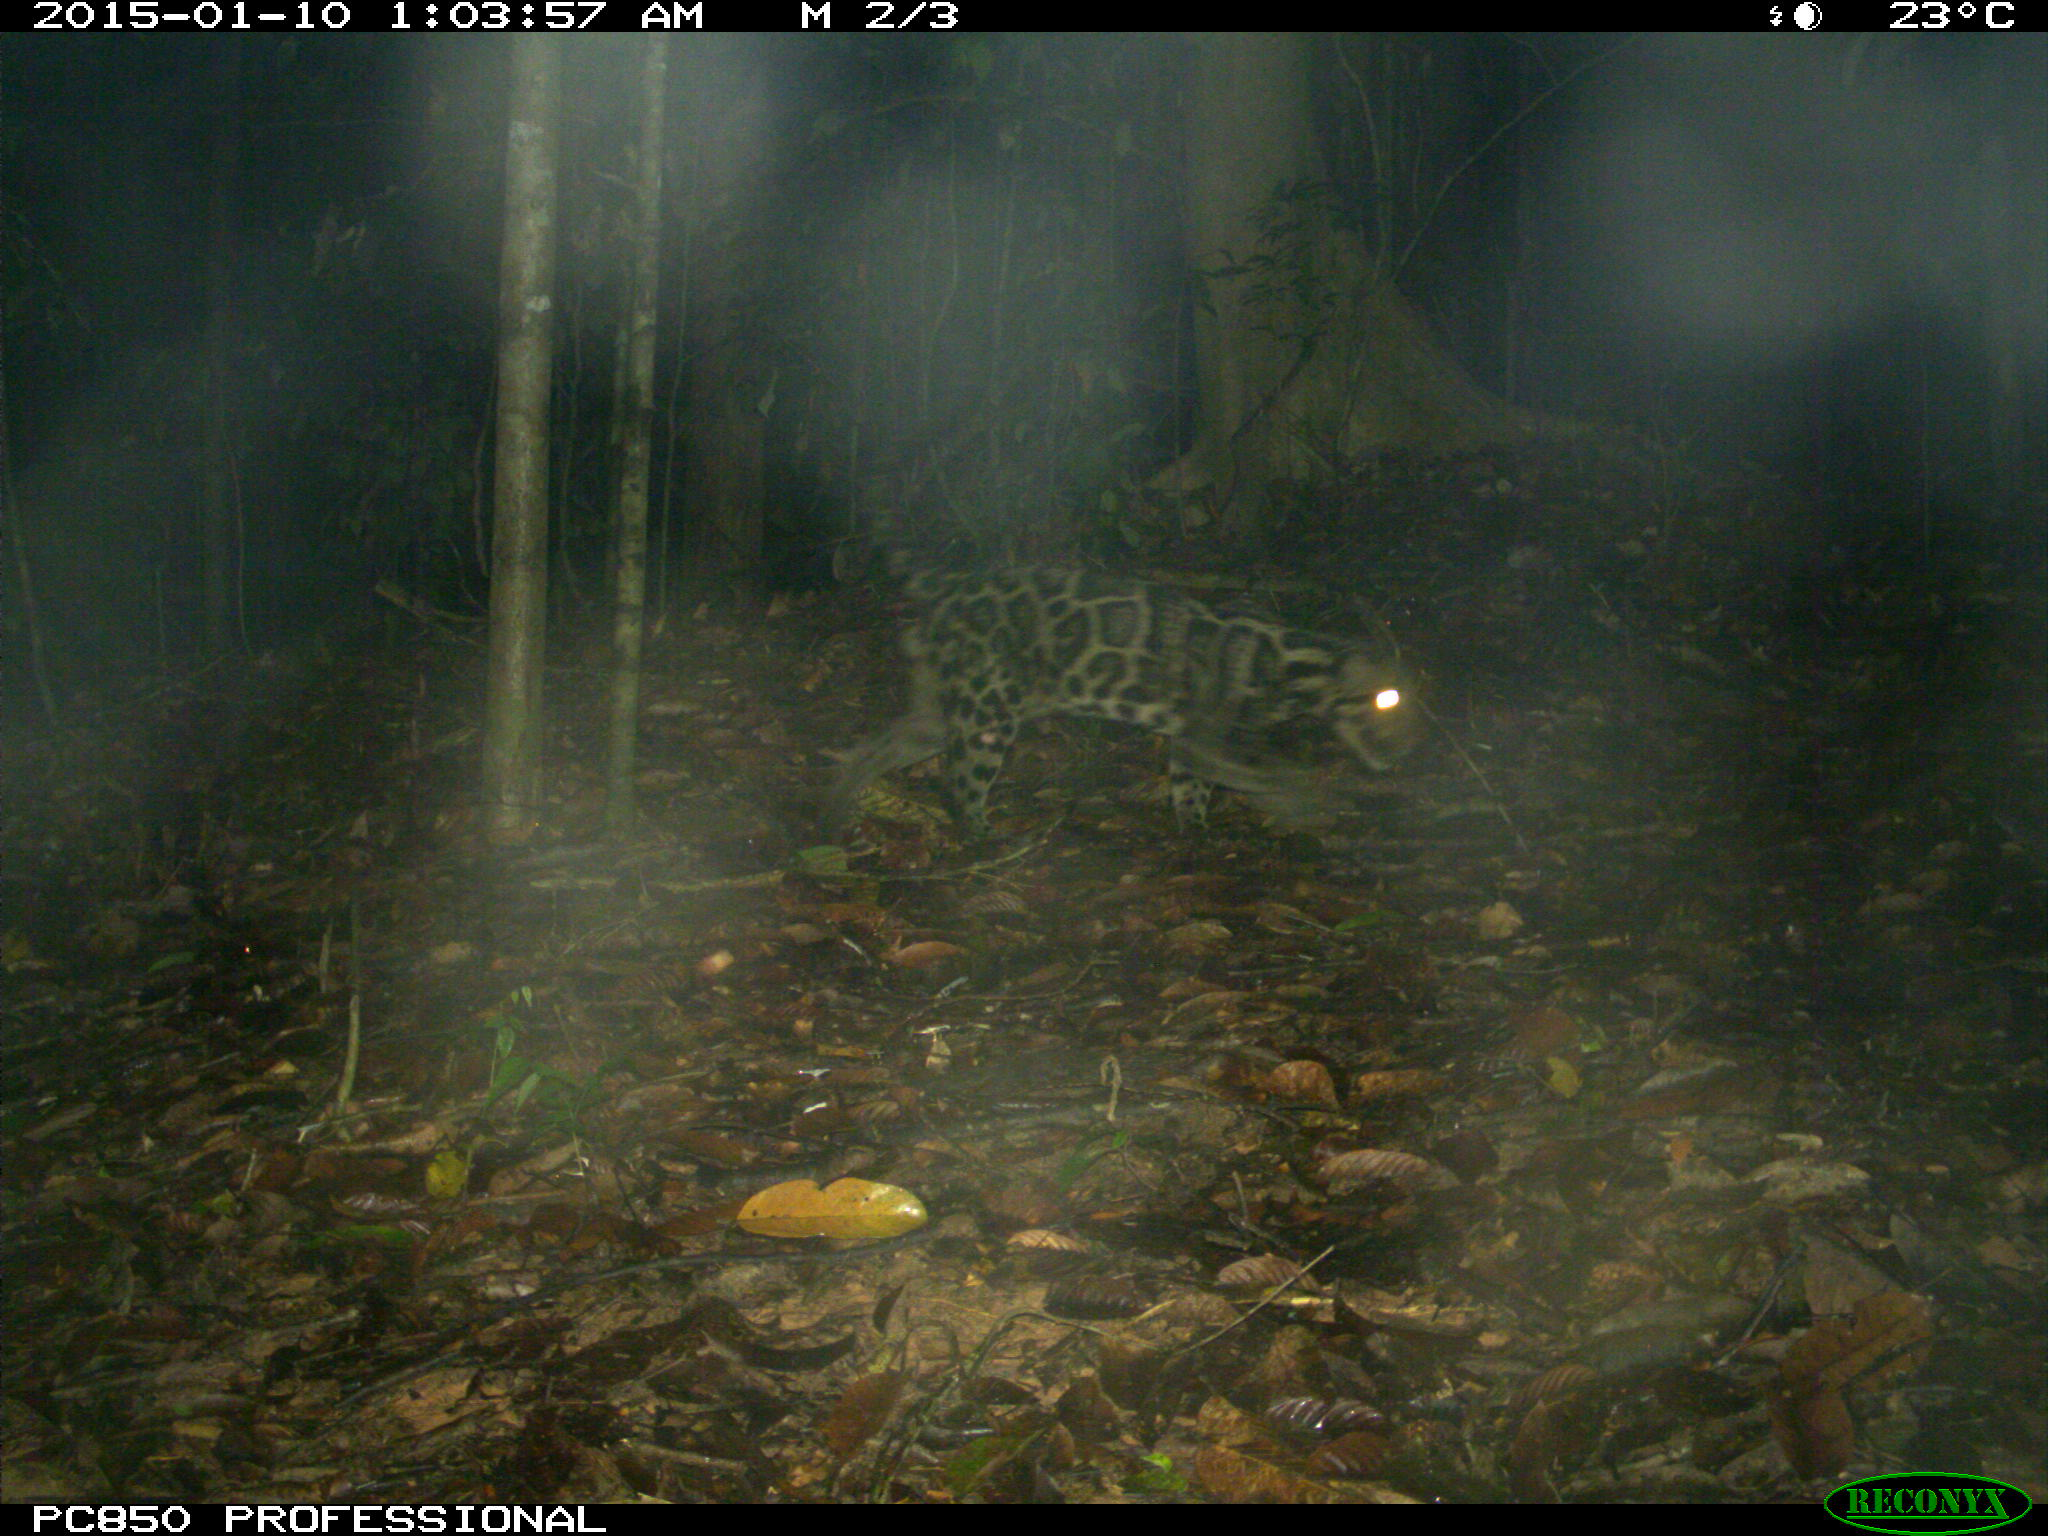
\includegraphics[width=\linewidth,height=.8\textheight,keepaspectratio]{images/example_DFR_5_male.JPG}
			\caption{DFR 5 male}
		\end{figure}
	\end{minipage}
\end{frame}

%-------------------------------------------------------

\begin{frame}{Bad Example Images}		
	\centering
	\begin{minipage}[c]{0.48\linewidth}
		\begin{figure}
			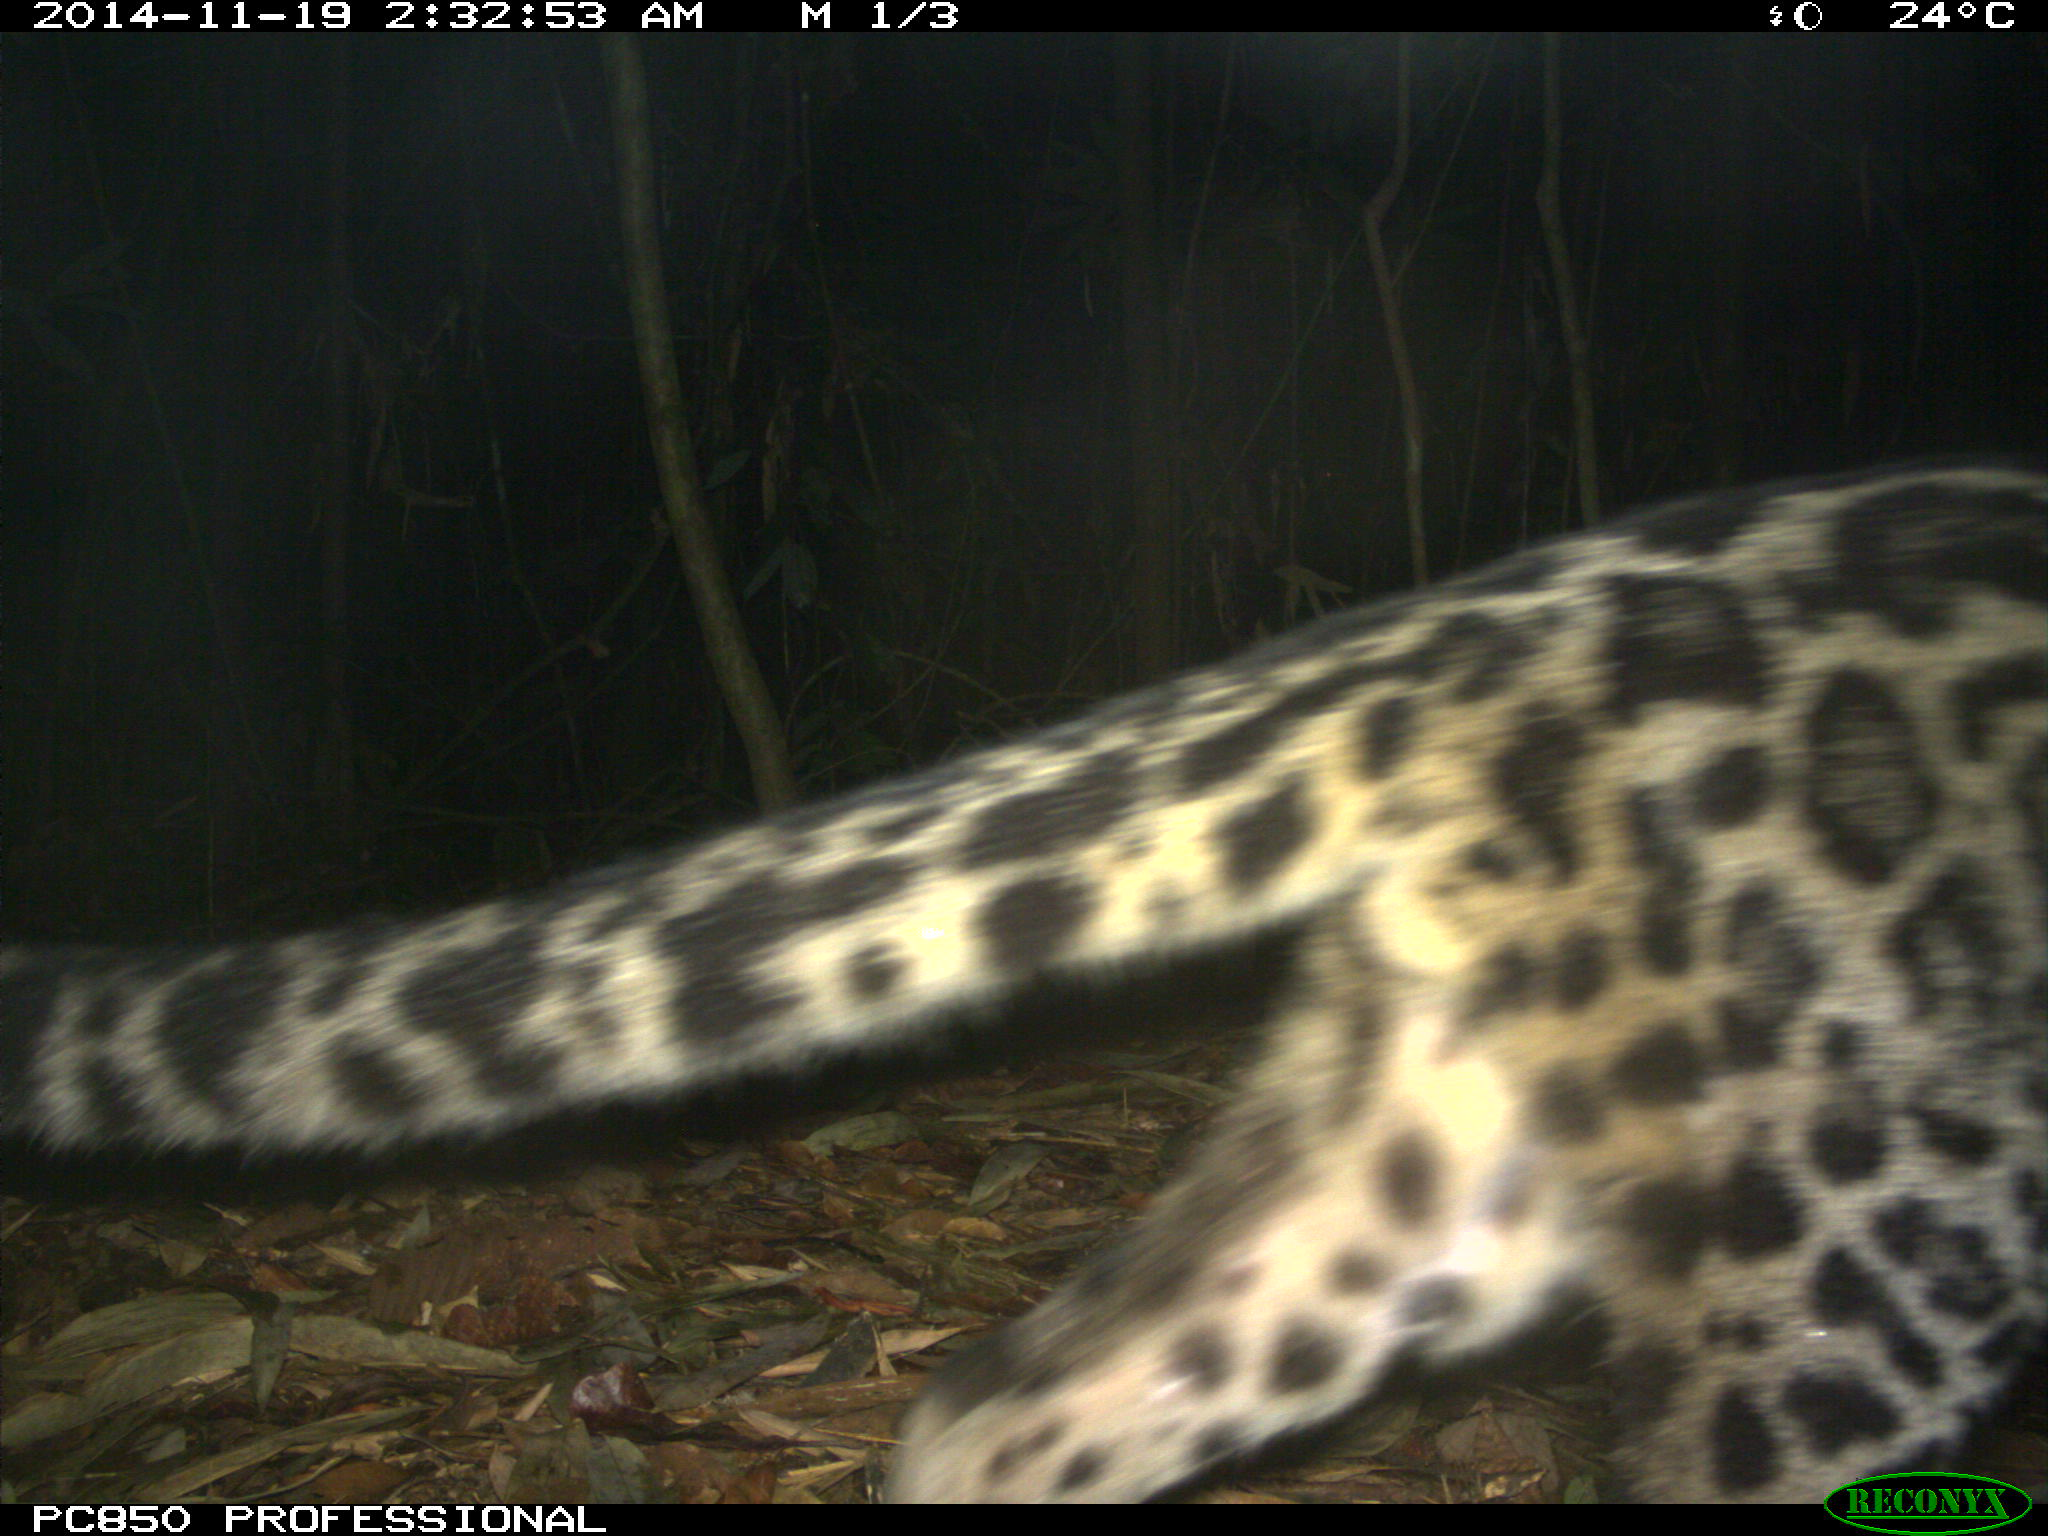
\includegraphics[width=.95\linewidth,height=\textheight,keepaspectratio]{images/example_bad_DFR_7_female.JPG}
			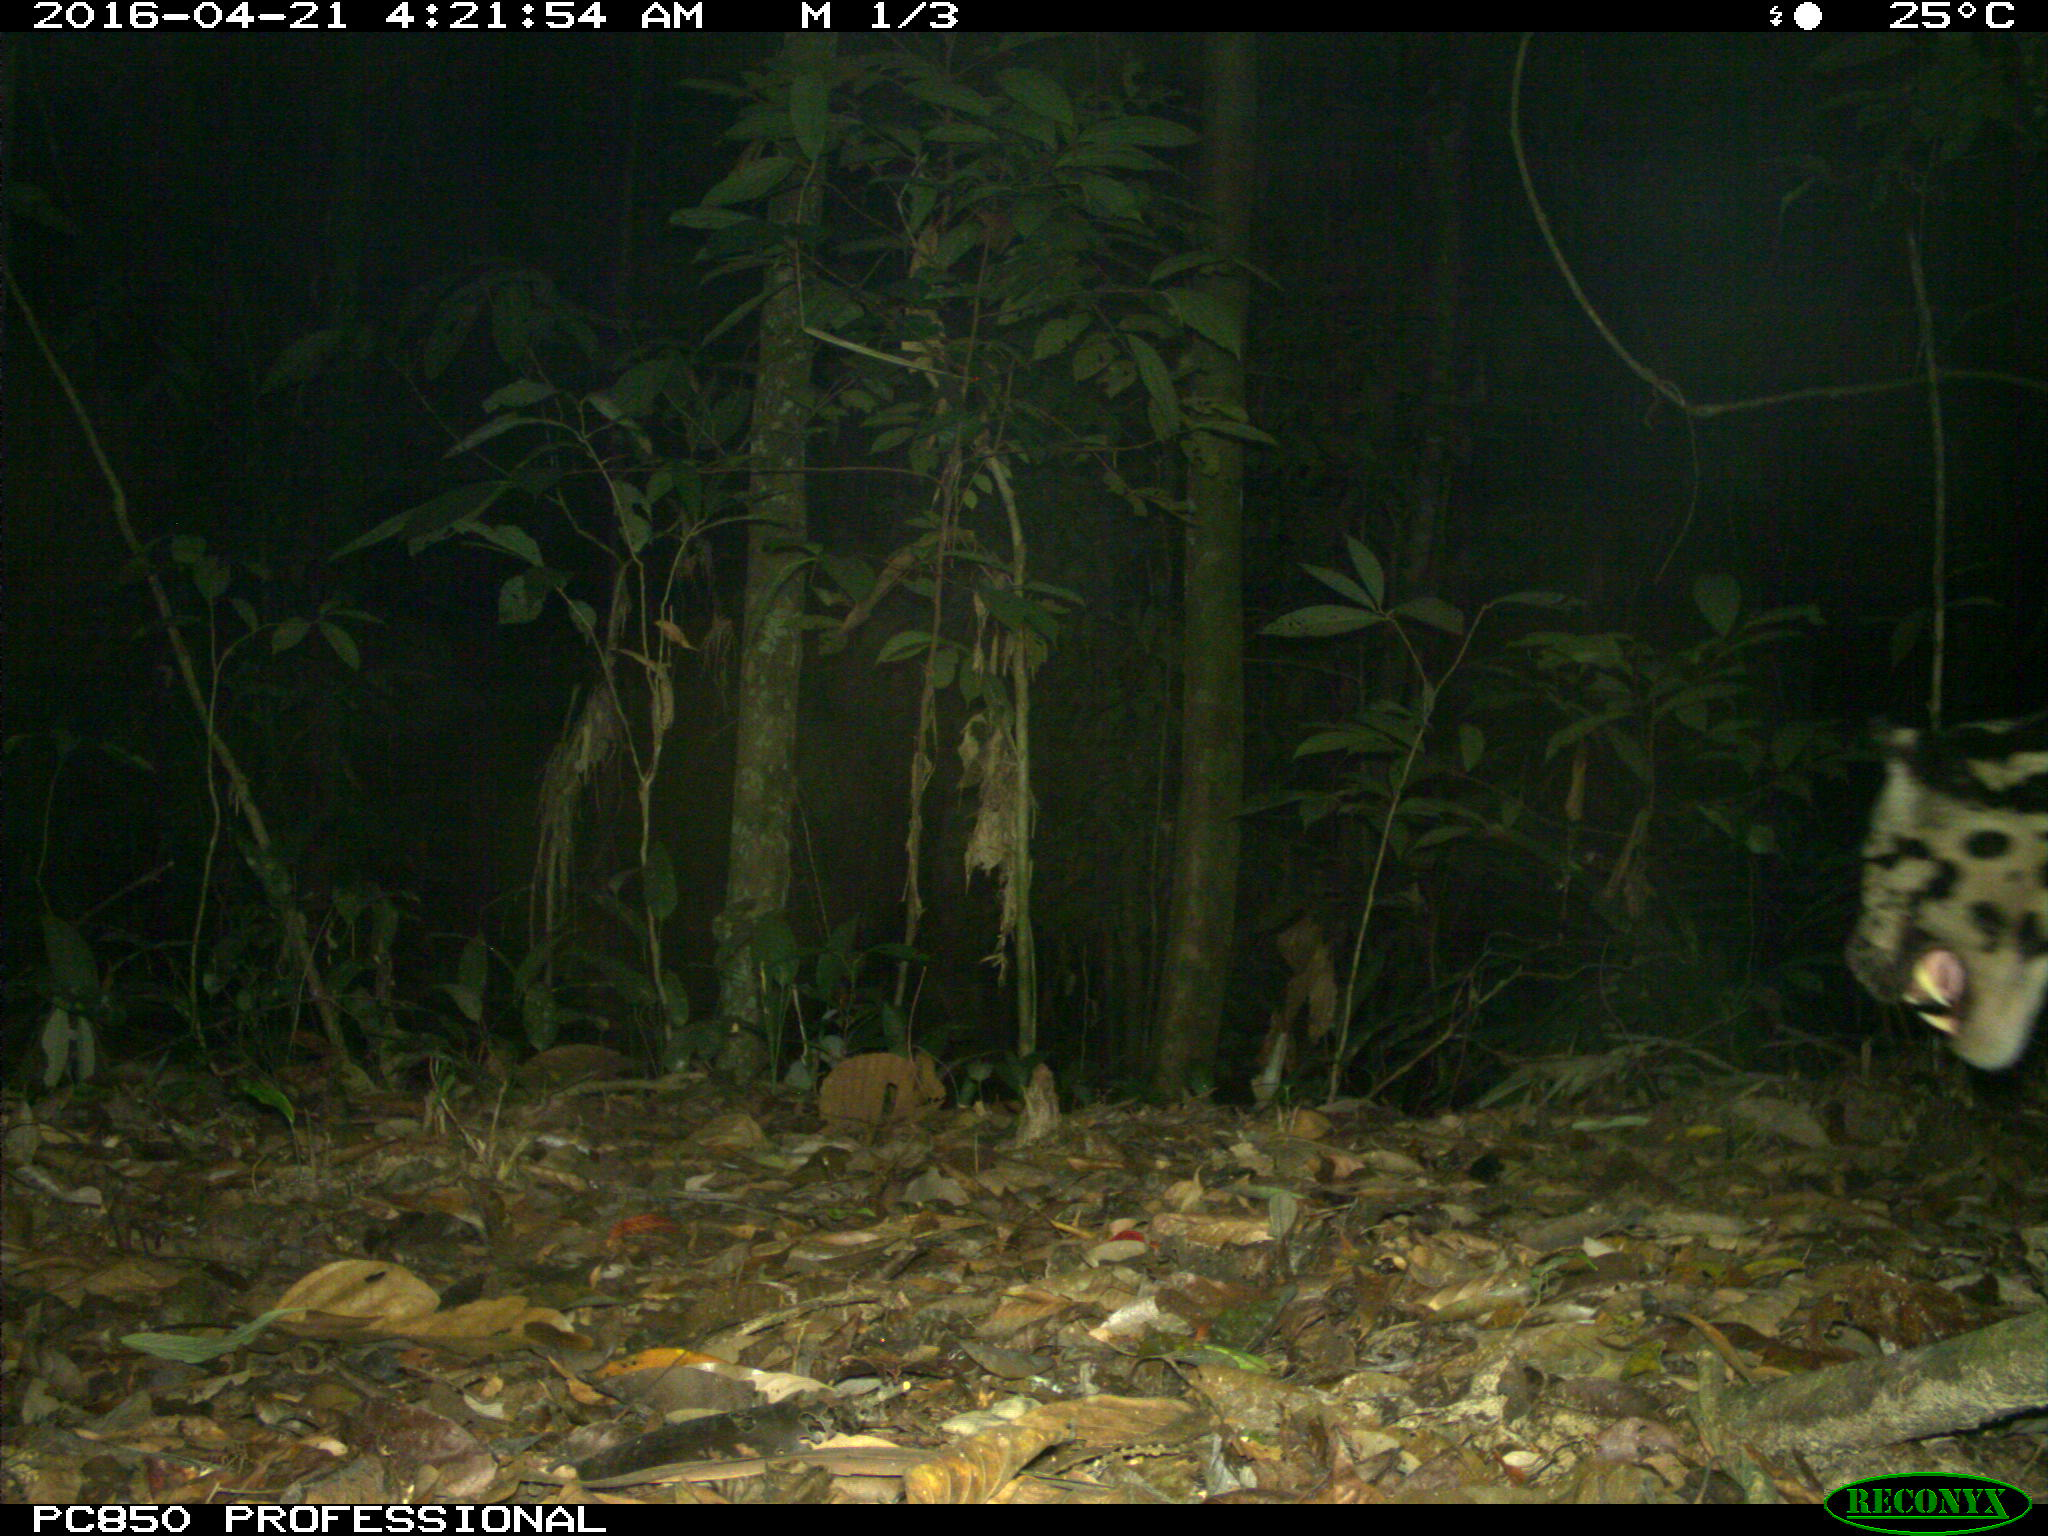
\includegraphics[width=.95\linewidth,height=\textheight,keepaspectratio]{images/example_bad_KFR_3_Male.JPG}
%			\caption{DFR 7 Female}
		\end{figure}
%		\begin{figure}
%			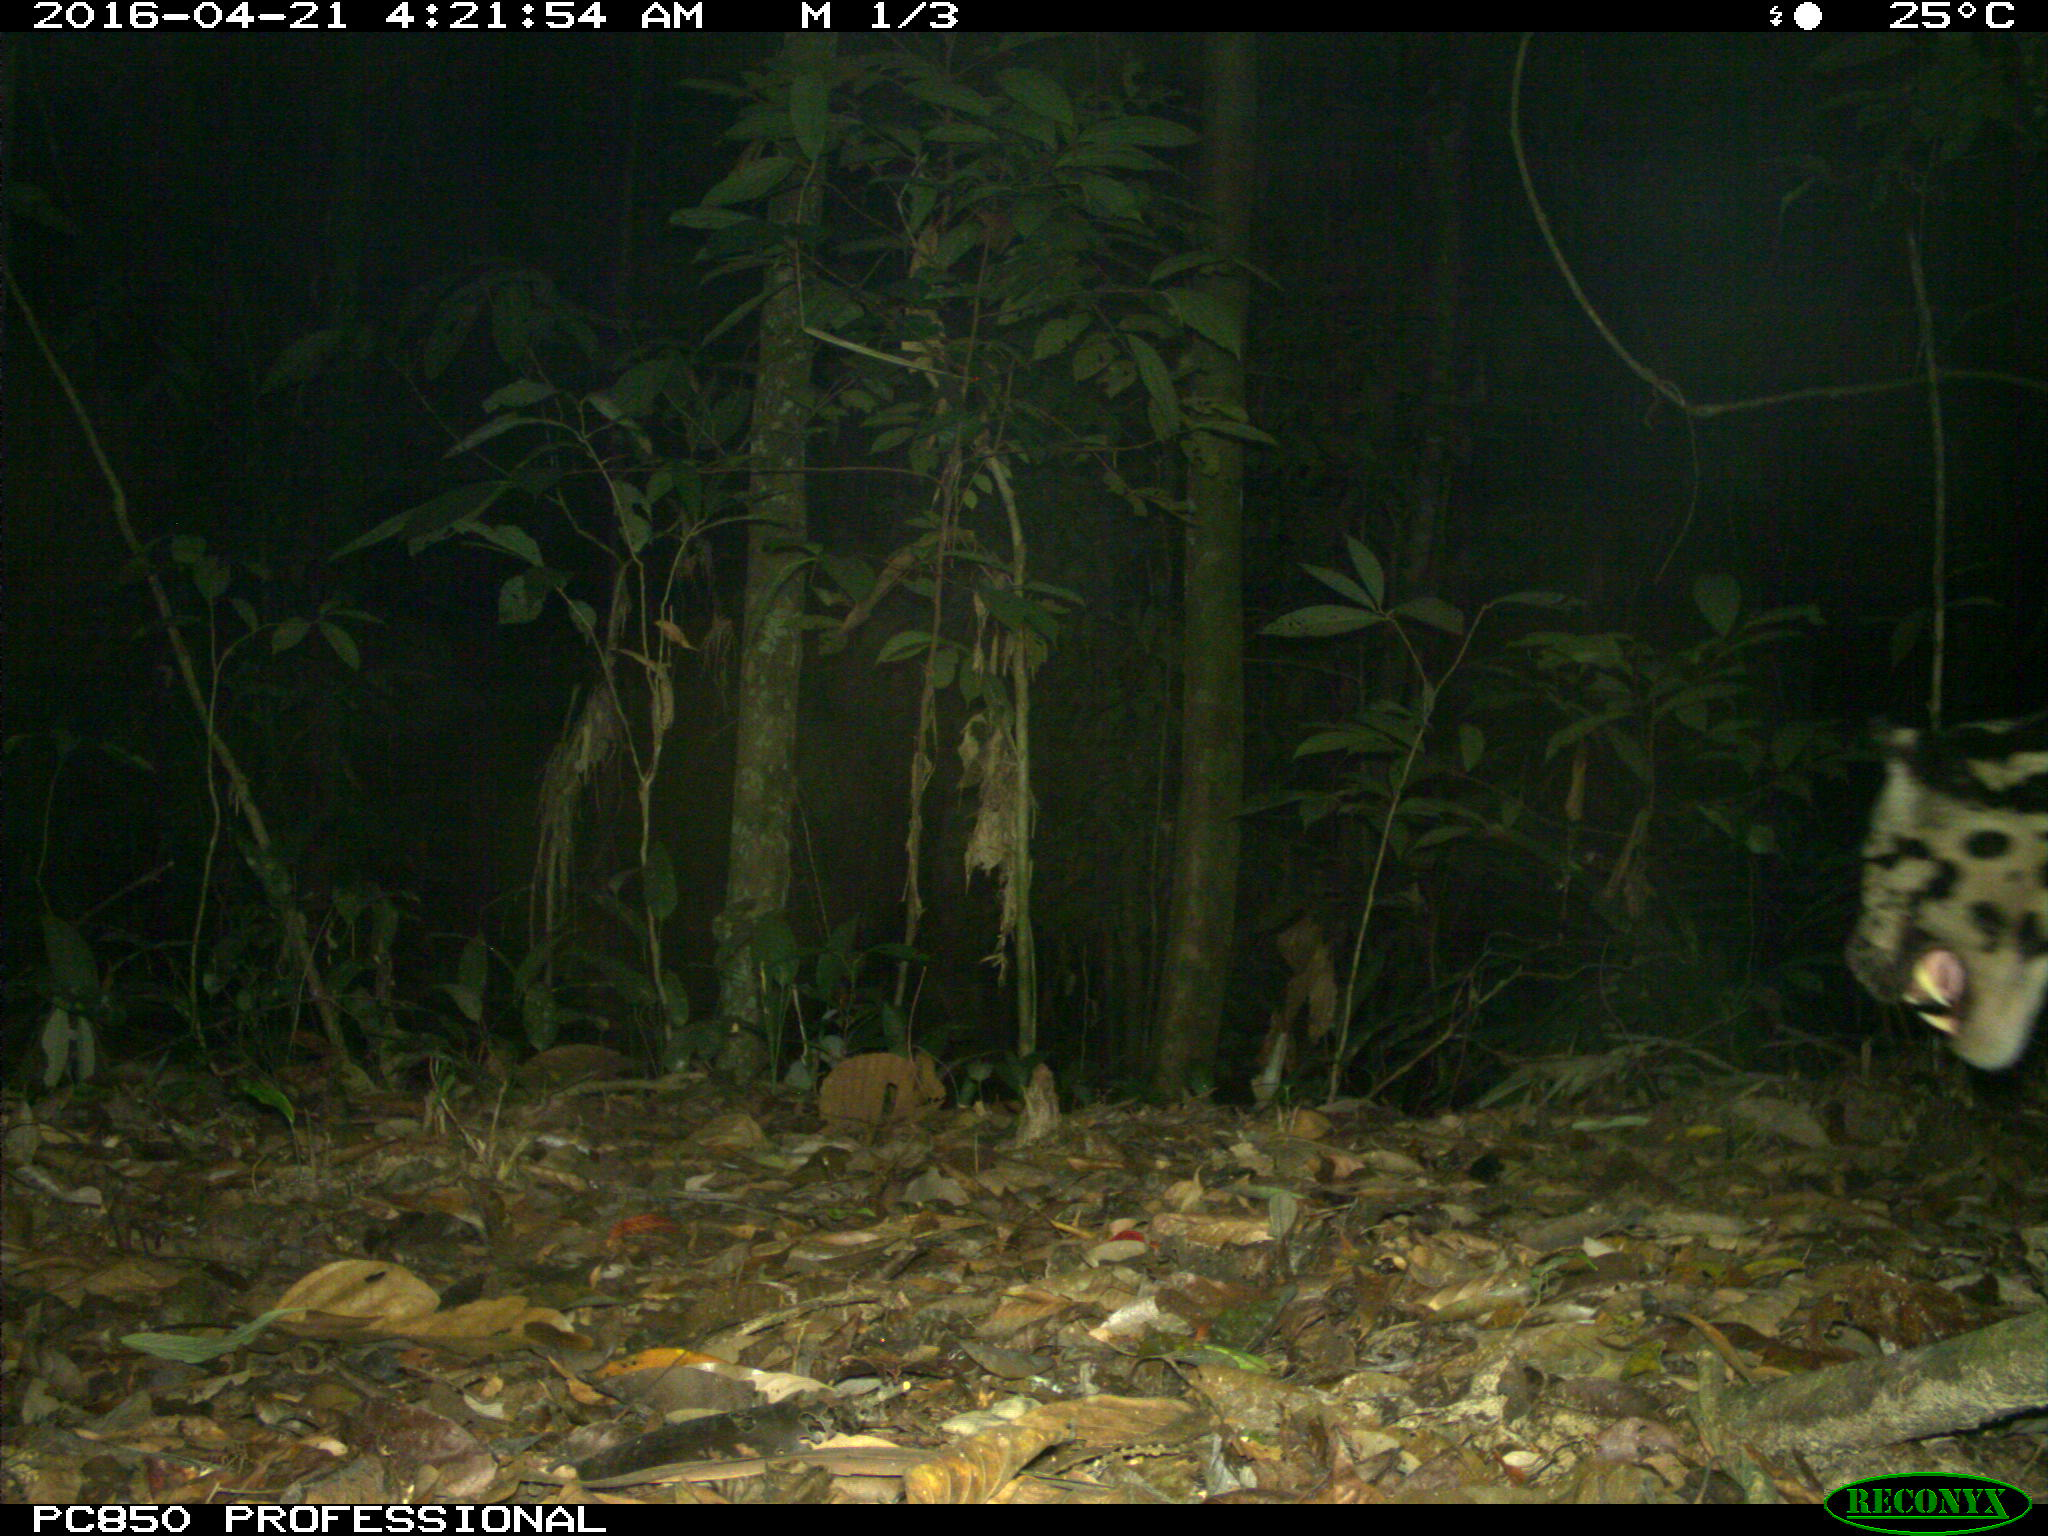
\includegraphics[width=\linewidth,height=\textheight,keepaspectratio]{images/example_bad_KFR_3_Male.JPG}
%%			\caption{KFR 3 Male}
%		\end{figure}
	\end{minipage}
	\hfill
	\begin{minipage}[c]{0.48\linewidth}
		\begin{figure}
			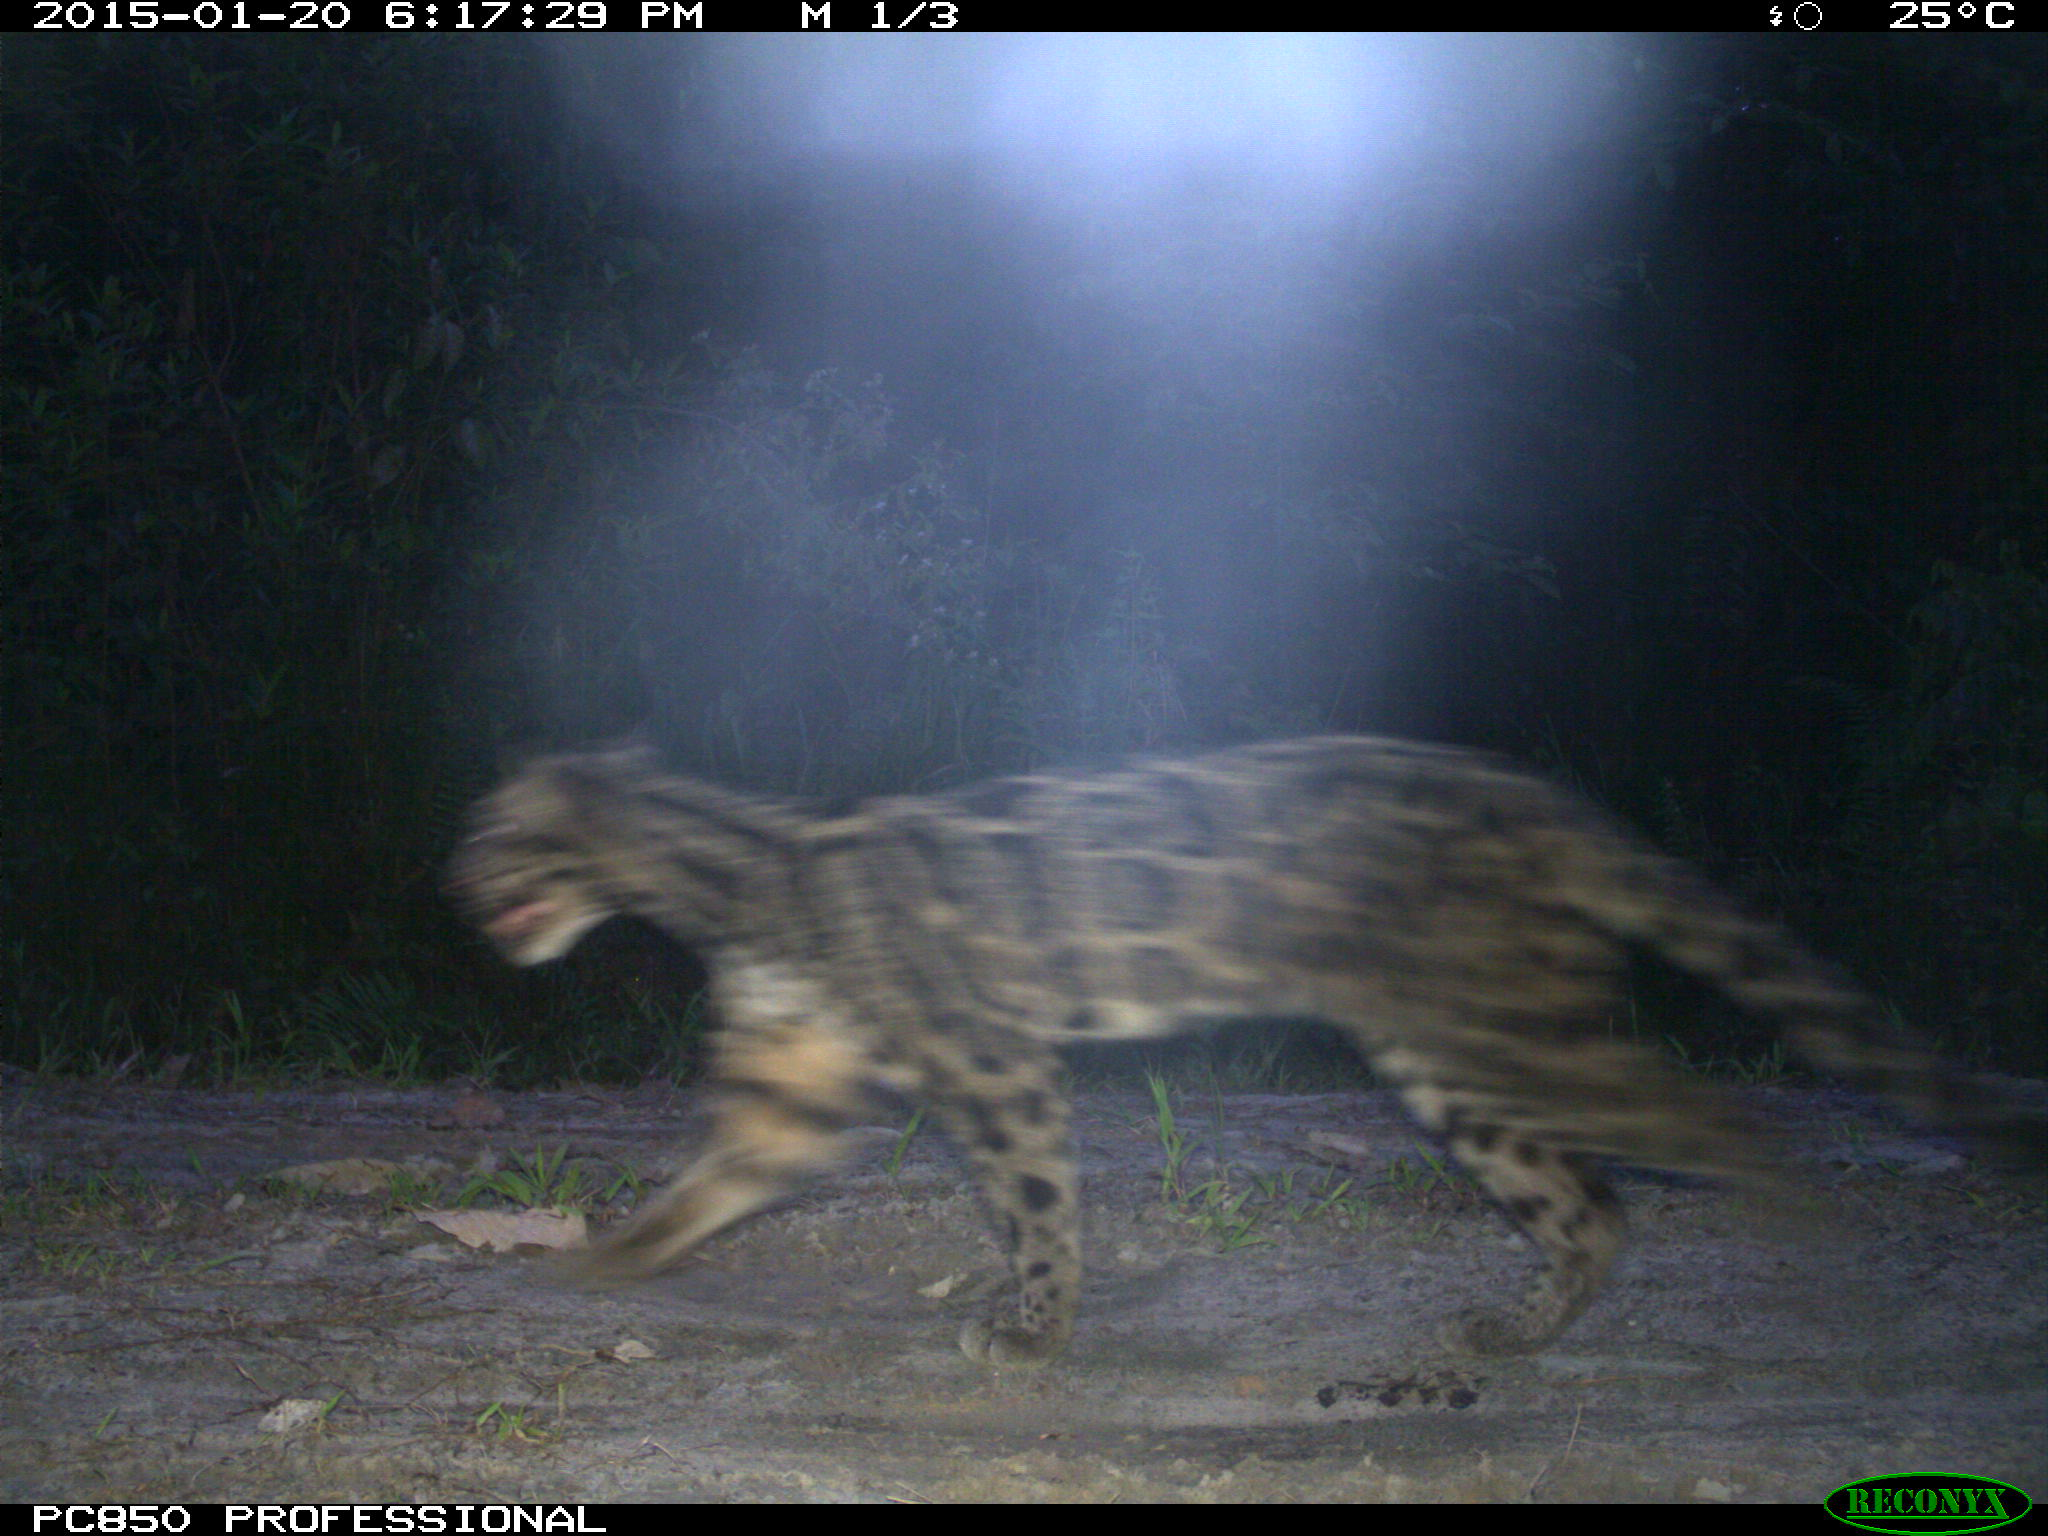
\includegraphics[width=\linewidth,height=\textheight,keepaspectratio]{images/example_bad_DFR_9_female.JPG}
%			\caption{DFR 9 Female}
		\end{figure}
	\end{minipage}
\end{frame}

%-------------------------------------------------------
\subsection{Architecture}
%-------------------------------------------------------

\begin{frame}{Architecture}
	\begin{figure}
		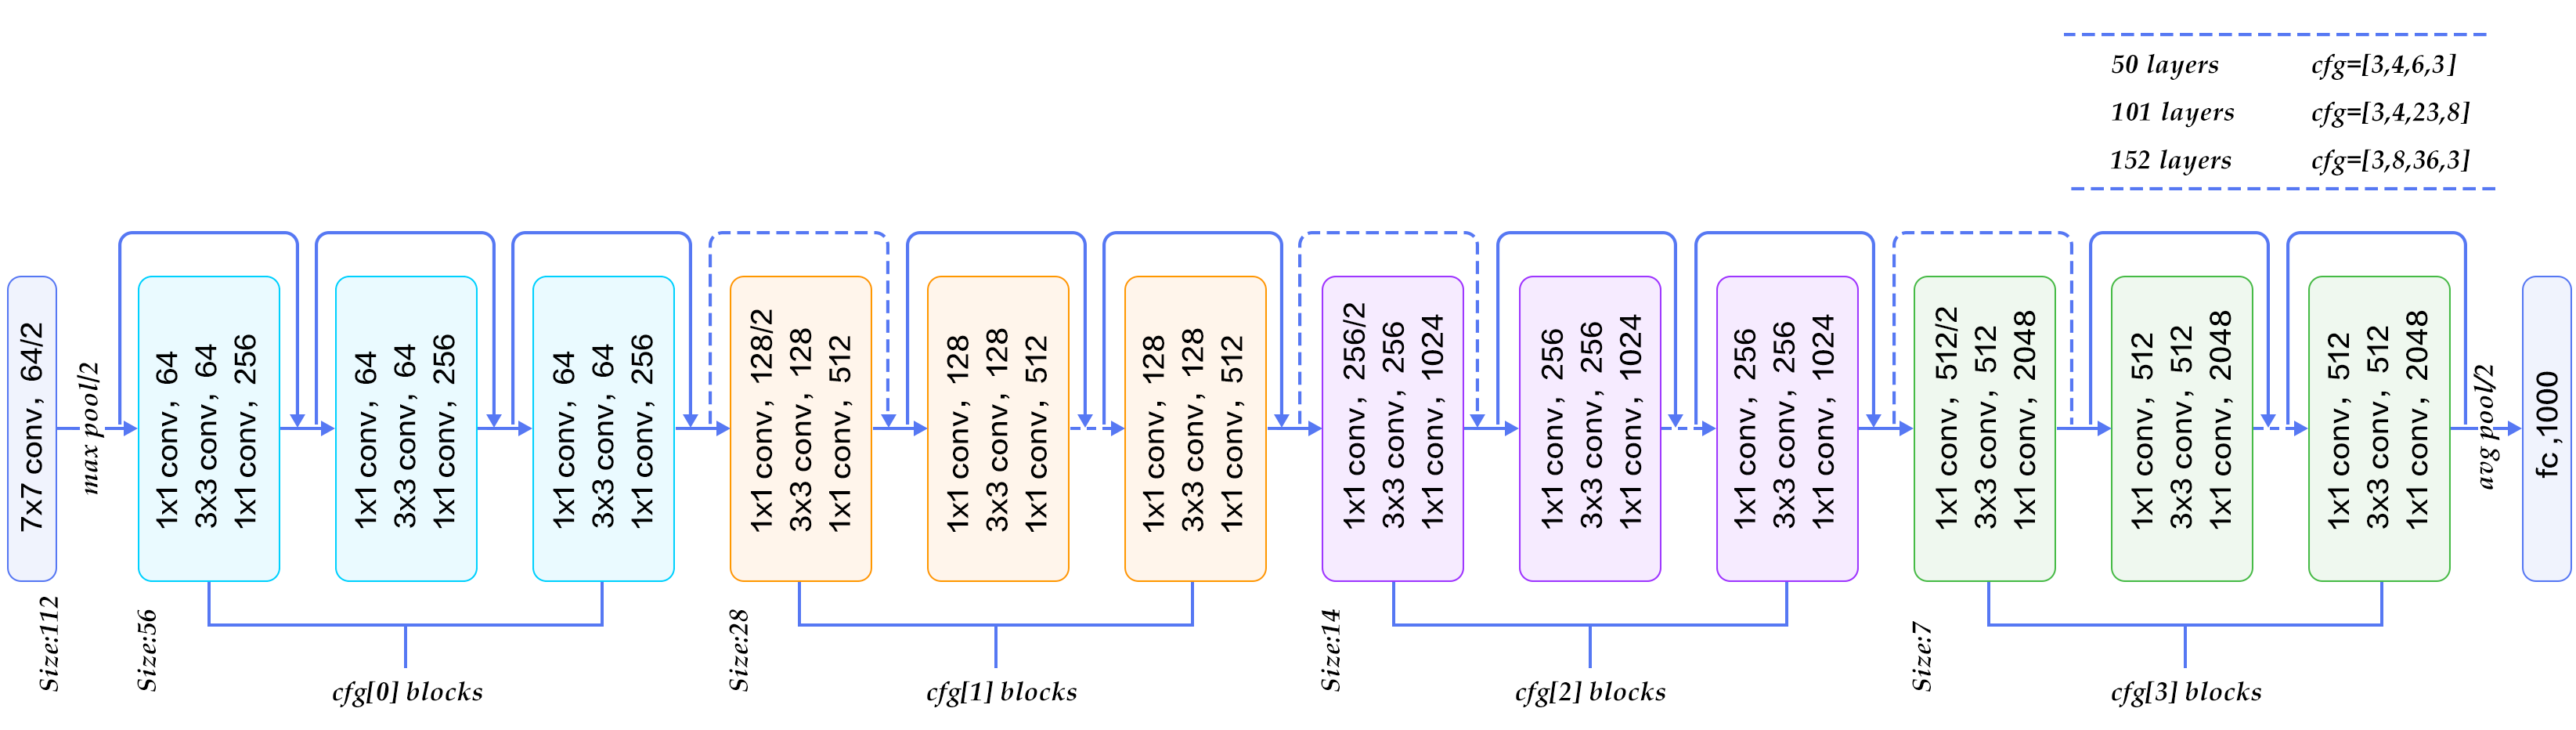
\includegraphics[width=\columnwidth]{images/resnet.png}
		\caption{ResNet Architecure}
	\end{figure}

	\begin{itemize}
		\item ResNet-18, ResNet-34 from scratch
		\item ResNet-50 finetuning
	\end{itemize}
\end{frame}

%-------------------------------------------------------
\subsection{Results}
%-------------------------------------------------------

\begin{frame}{Scores}
	Insert Scores and conf mat here
\end{frame}
%-------------------------------------------------------

\begin{frame}{Results}
	\begin{figure}
		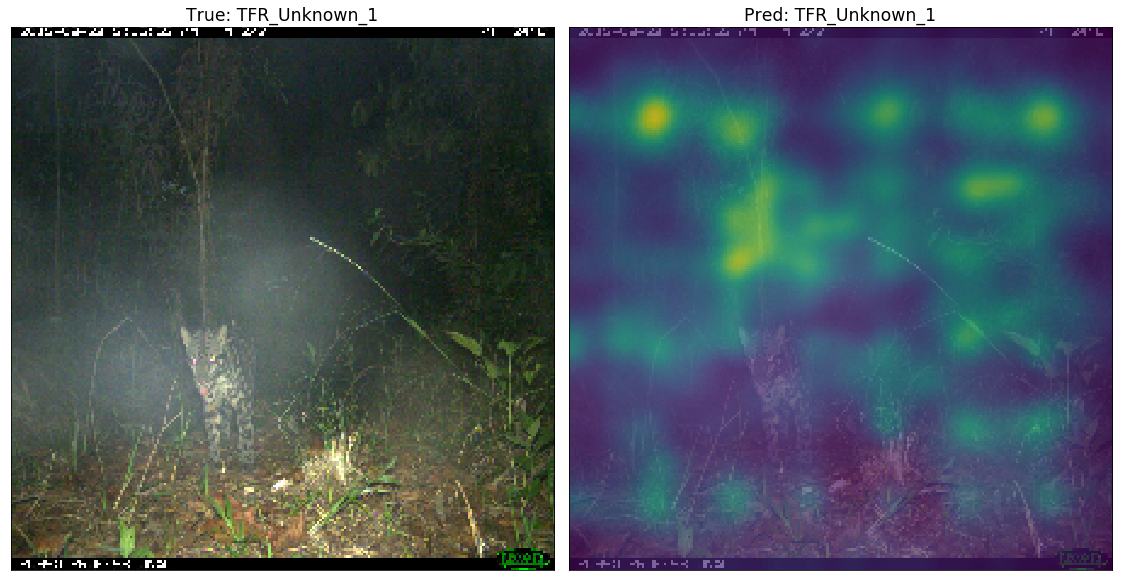
\includegraphics[width=\columnwidth]{images/result_leo_1.png}
		\caption{Network Attention}
	\end{figure}
\end{frame}

%-------------------------------------------------------


\begin{frame}{Results}
	\begin{figure}
		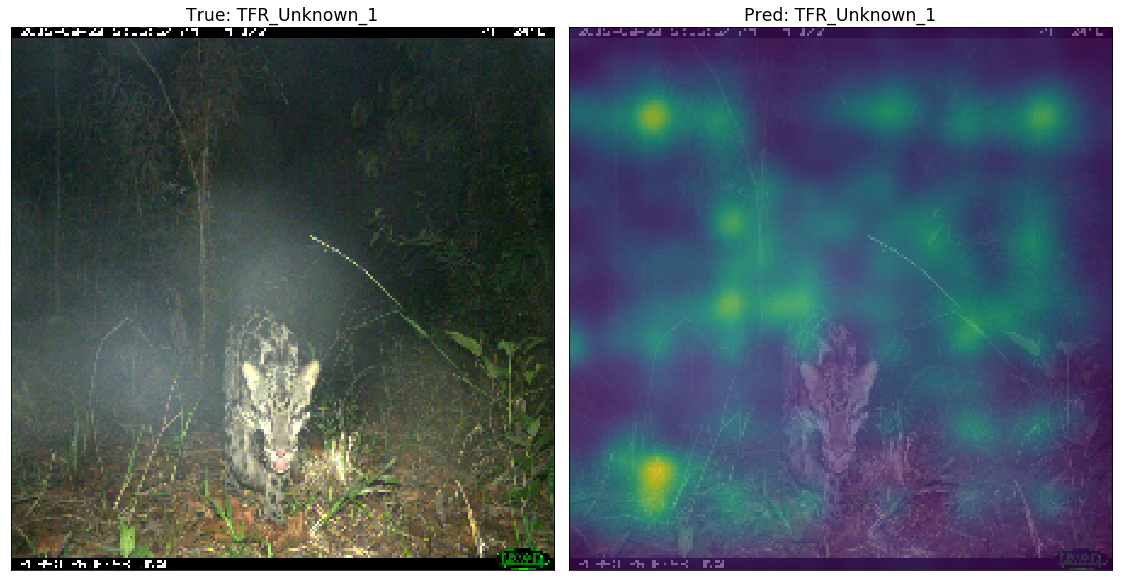
\includegraphics[width=\columnwidth]{images/result_leo_2.png}
		\caption{Network Attention}
	\end{figure}
\end{frame}

%-------------------------------------------------------

\begin{frame}{Training Process}
	\begin{figure}
		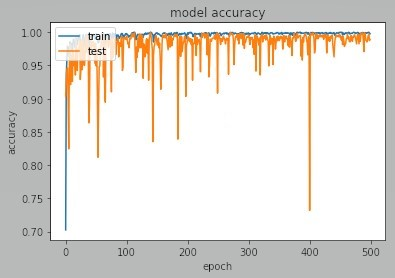
\includegraphics[width=.9\columnwidth,height=\textheight,keepaspectratio]{images/Pretrain_acc_ResNet50_cropped_heavy_augment_lr0_0001.jpg}
		\caption{Accuracy development}
	\end{figure}
\end{frame}

%-------------------------------------------------------

%\begin{frame}{Results}
%	\begin{figure}
%		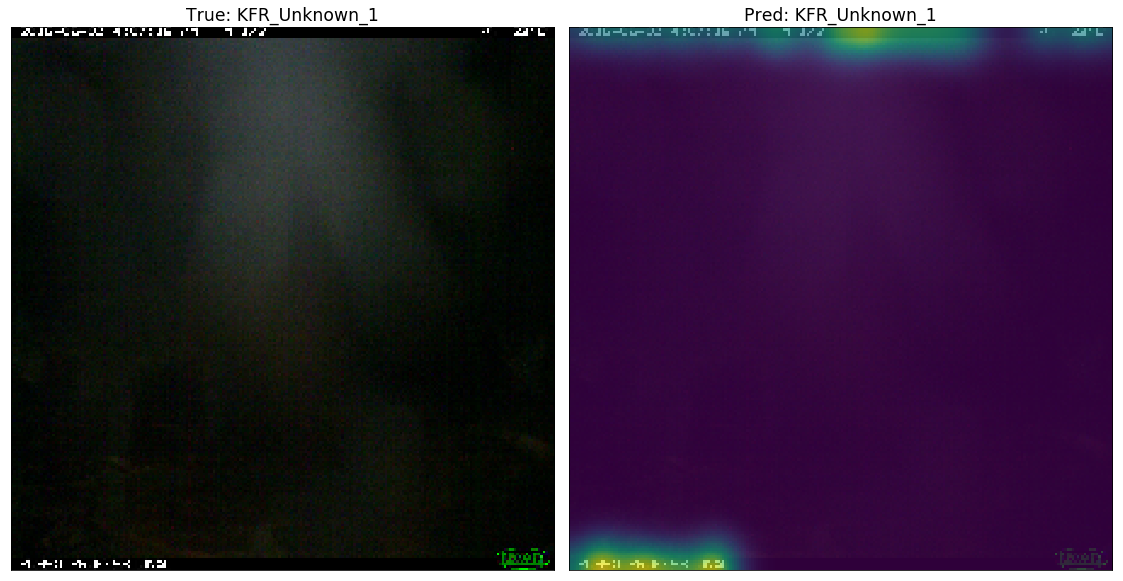
\includegraphics[width=\columnwidth]{images/Attention_Leo_Stamp.png}
%		\caption{Network Attention}
%	\end{figure}
%\end{frame}
%-------------------------------------------------------

\begin{frame}{Results}
	\begin{figure}
		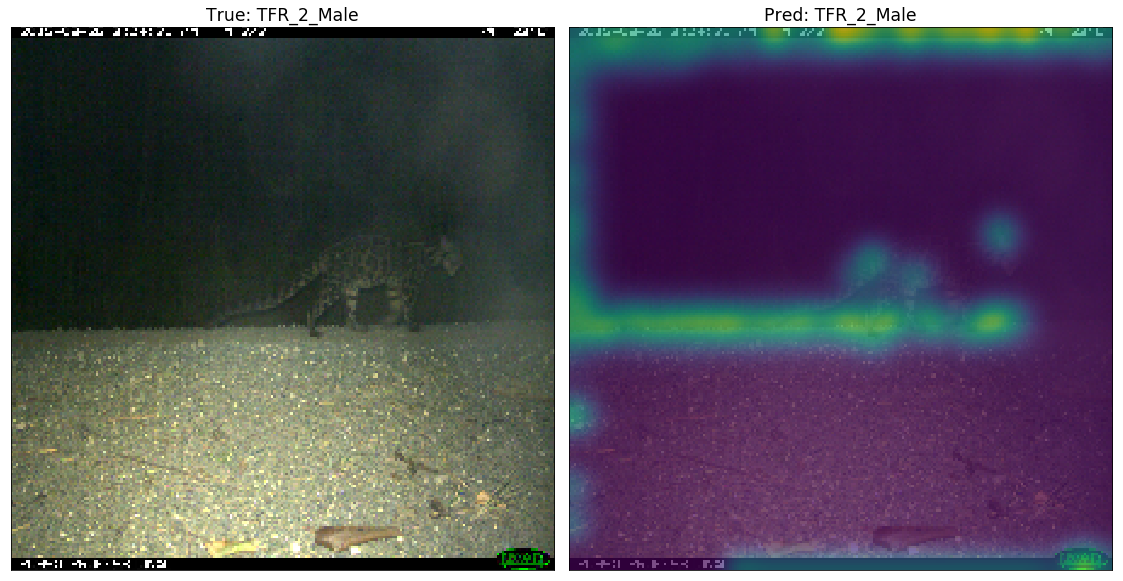
\includegraphics[width=\columnwidth]{images/Attention_Leo_Stamp2.png}
		\caption{Network attention on logo and time stamp}
	\end{figure}
\end{frame}

%-------------------------------------------------------
\subsection{Alternative Approach}
\begin{frame}{Using Bounding Boxes}
	\begin{figure}
		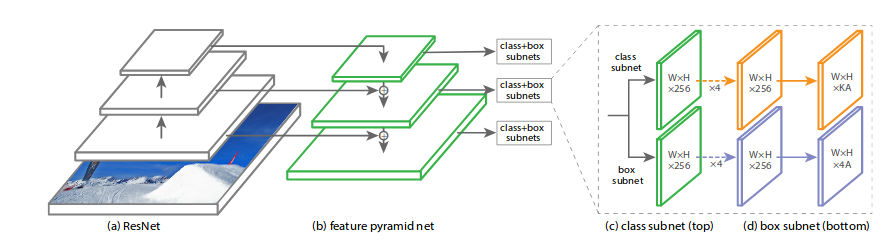
\includegraphics[width=\columnwidth]{images/retinanet.png}
		\caption{ResNet Architecure}
	\end{figure}

	\begin{itemize}
		\item losses semantic information an detect small objects RPN
		\item used prefered backbone
		\item extract after each pooling layer feature maps -- Feature pyramid network based on resnet

	\end{itemize}
\end{frame}

%-------------------------------------------------------

\begin{frame}{Scores}
	Insert Scores and conf mat here
\end{frame}
%-------------------------------------------------------

\begin{frame}{Results}
	\begin{figure}
		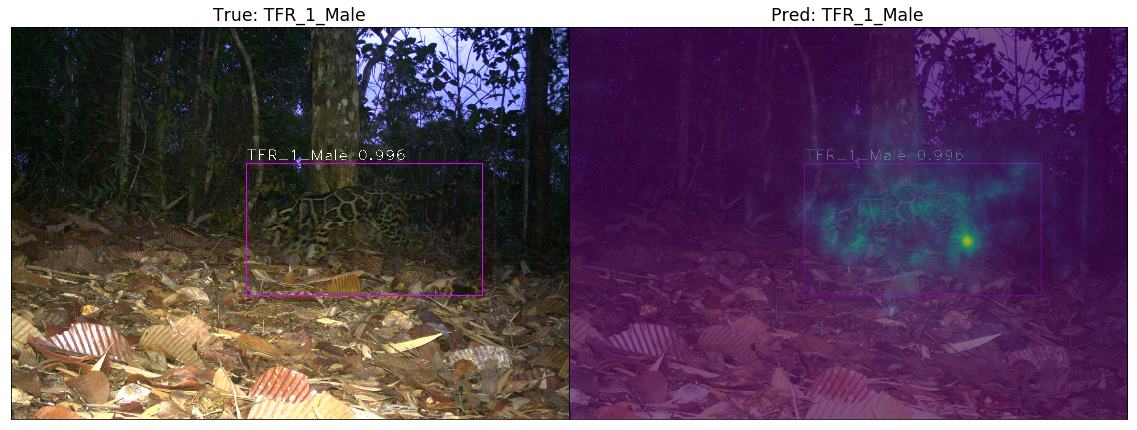
\includegraphics[width=\columnwidth]{images/RetinaNet_Attention_correct_good_quality2.png}
		\caption{Network attention on logo and time stamp}
	\end{figure}
\end{frame}

%-------------------------------------------------------

\begin{frame}{Results}
	\begin{figure}
		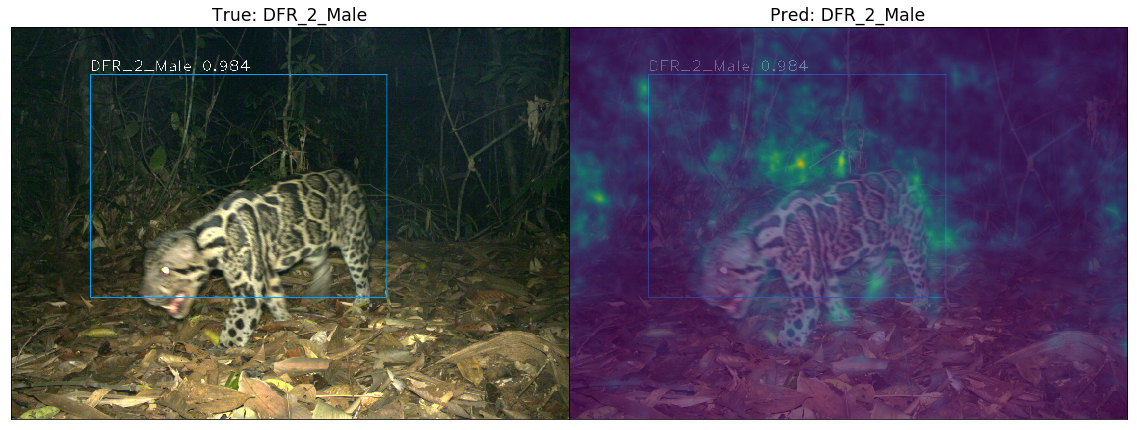
\includegraphics[width=\columnwidth]{images/RetinaNet_No_Attention_correct2.png}
		\caption{Network attention on logo and time stamp}
	\end{figure}
\end{frame}

%-------------------------------------------------------
\section{Problem 2: Classification of Species}
%-------------------------------------------------------
\subsection{Data Set}
%-------------------------------------------------------
\begin{frame}{Data Set}
	\begin{minipage}[c]{0.48\linewidth}
		\centering
		\begin{figure}
			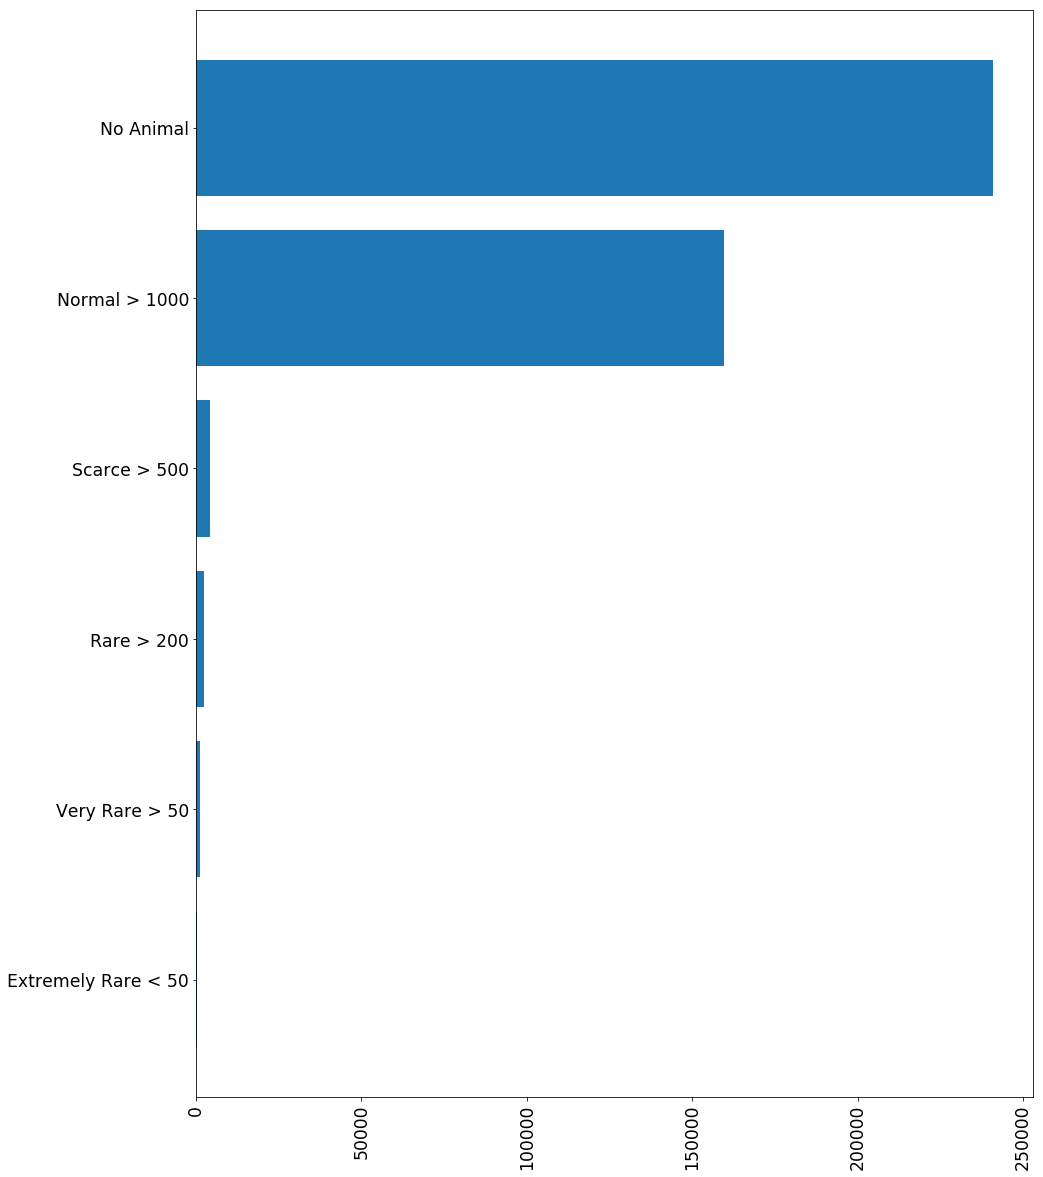
\includegraphics[width=\linewidth,height=.8\textheight,keepaspectratio]{images/Data_dist_sorted_reduced_v2.png}
			\caption{ResNet Architecure}
		\end{figure}
	\end{minipage}
	\hfill
	\begin{minipage}[c]{0.48\linewidth}
	\begin{itemize}
		\item 87 Classes
	\end{itemize}

	\end{minipage}
\end{frame}

%-------------------------------------------------------

%\begin{frame}[allowframebreaks]{Bibliography}
%		\bibliographystyle{abbrv}
%		\bibliography{bibliography}
%		
%		% abstract 
%		\nocite{ichikawa:2002}
%		\nocite{Hao:2012}
%		\nocite{buono:2007}
%		\nocite{boegl:2013}
%		\nocite{boegl:2014}
%		\nocite{steed:2017}
%		
%		% spatial
%		\nocite{maciejewski:2011}
%		\nocite{Andrienko:2010:Space}
%\end{frame}

%-------------------------------------------------------

{\1
\begin{frame}[plain,noframenumbering]
  \finalpage{Thank you for listening}
\end{frame}}

\end{document}